\documentclass[tikz,border=10pt]{standalone}
\usepackage{amsmath}
\usepackage{amssymb}
\usepackage{tikz}
\usetikzlibrary{arrows.meta,calc,decorations.pathreplacing,decorations.pathmorphing,patterns,shapes.geometric,positioning,shadings}

\begin{document}
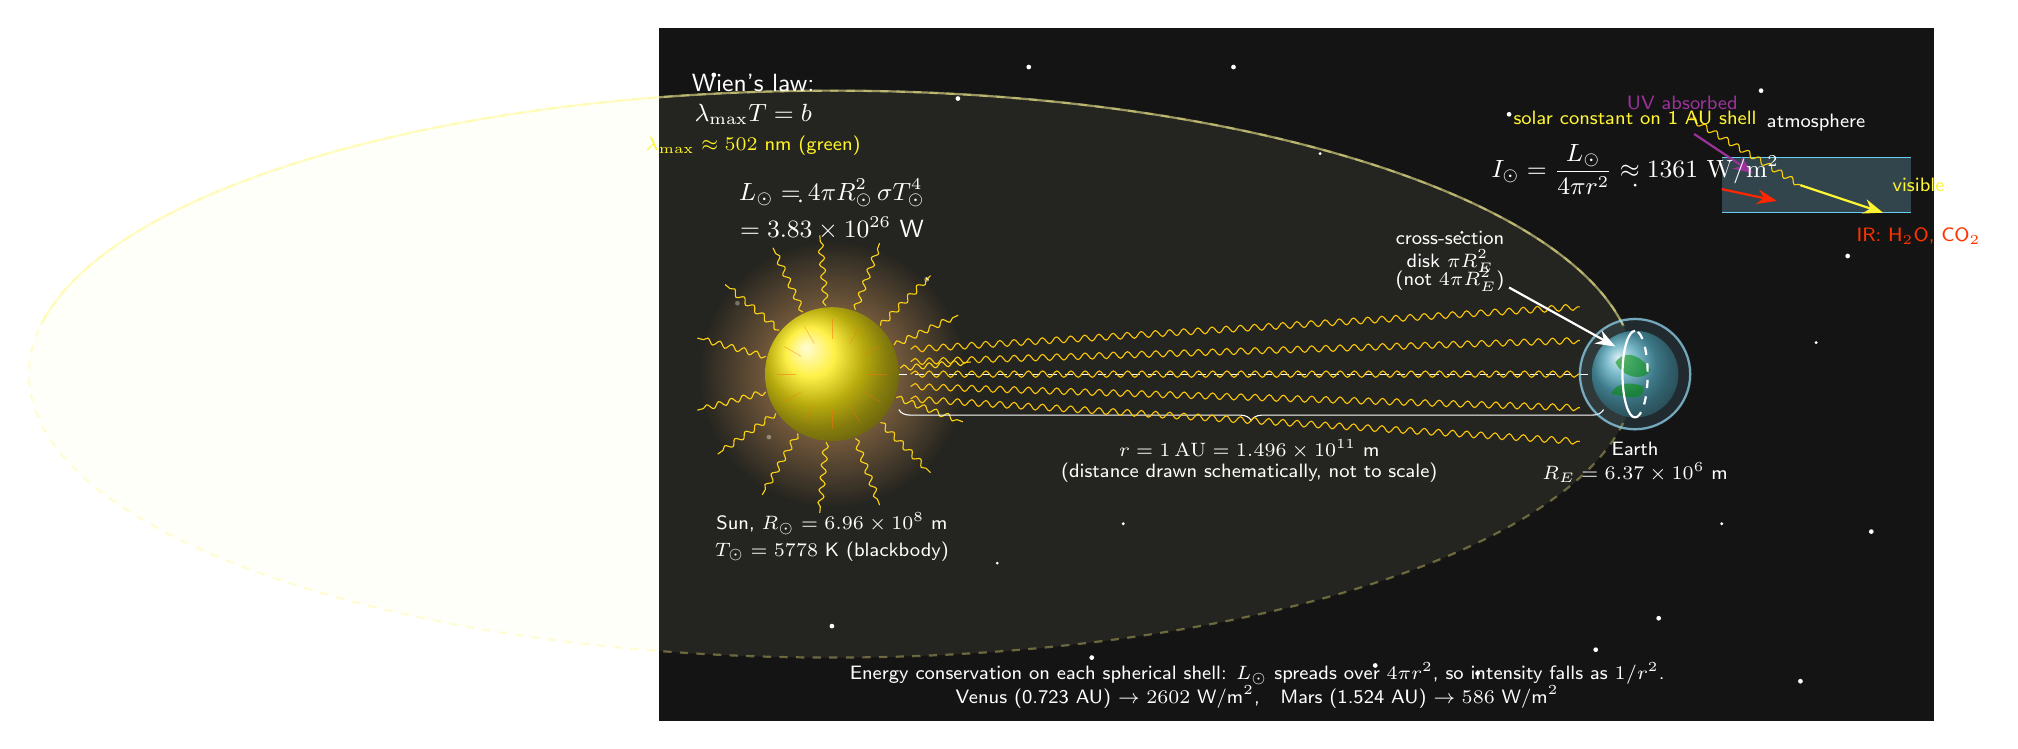
\begin{tikzpicture}[
    >={Stealth[length=2.5mm]},
    font=\sffamily\small,
    wave/.style={yellow!70!orange, thin, decorate, decoration={snake, amplitude=0.35mm, segment length=1.6mm}},
    wavelong/.style={yellow!60!orange, thin, decorate, decoration={snake, amplitude=0.4mm, segment length=1.8mm}},
    whitearrow/.style={->, white, thick},
    note/.style={font=\sffamily\scriptsize, text=white!85},
    formula/.style={font=\sffamily\small, text=white},
]

% ===== dark cosmic background =====
\fill[black!92] (-7.6,-4.4) rectangle (8.6,4.4);
% starry background
\foreach \s in {(-6.9,3.8),(-5.4,-3.2),(-3.8,3.5),(-2.1,-3.6),(-0.3,3.9),(1.5,-3.7),(3.2,3.3),(5.1,-3.1),(6.4,3.6),(7.8,-2.0),(-6.2,-0.8),(-4.2,1.2),(7.5,1.5),(-6.6,0.9),(4.3,-3.5),(2.8,-3.8),(6.9,-3.9),(-2.9,3.9)}
  \fill[white!90] \s circle (0.03);
\foreach \s in {(-5.8,2.2),(-3.3,-2.4),(0.8,2.8),(2.6,1.8),(4.8,2.4),(5.9,-1.9),(-1.7,-1.9),(7.1,0.4)}
  \fill[white!60] \s circle (0.02);

% ===== SUN (left) =====
\begin{scope}[shift={(-5.4,0)}]
  % corona glow
  \shade[inner color=orange!60, outer color=black!92, opacity=0.7] (0,0) circle (1.7);
  % sun body
  \shade[ball color=yellow!85!orange] (0,0) circle (0.85);
  % surface texture
  \foreach \a in {0,30,60,...,330}
    \draw[orange!80!red, very thin, opacity=0.5] (0,0) ++(\a:0.55) ++(\a:-0.1) -- ++(\a:0.25);
  % radial rays (light emitted in all directions)
  \foreach \a in {5,25,45,70,95,115,140,165,195,215,240,265,290,315,340}
    \draw[wave] (0,0) ++(\a:0.87) -- ++(\a:0.9);

  % label "Sun"
  \node[note] at (0,-1.9) {Sun, $R_\odot = 6.96\times 10^{8}$ m};
  \node[note] at (0,-2.25) {$T_\odot = 5778$ K (blackbody)};

  % luminosity formula
  \node[formula, align=center] at (0,2.3)
    {$L_\odot = 4\pi R_\odot^2\,\sigma T_\odot^4$};
  \node[formula, align=center] at (0,1.85)
    {$= 3.83\times 10^{26}$ W};
\end{scope}

% ===== 1 AU spherical shell (semi-transparent) =====
\begin{scope}
  % full ellipse as dashed outline of the shell (the 1 AU sphere)
  \draw[yellow!50!white, opacity=0.35, thick, dashed]
    (-5.4,0) ellipse (10.2 and 3.6);
  % top front highlight
  \draw[yellow!40!white, opacity=0.55, thick]
    (-5.4,0) ++(10:10.2 and 3.6) arc (10:170:10.2 and 3.6);
  % fill hint
  \fill[yellow!25, opacity=0.07]
    (-5.4,0) ellipse (10.2 and 3.6);
\end{scope}

% dashed radial line Sun -> Earth with 1 AU label
\draw[white!70, dashed, thin] (-4.55,0) -- (4.4,0);
\draw[white!75, thin, decorate, decoration={brace, amplitude=4pt, mirror}]
  (-4.55,-0.45) -- (4.4,-0.45);
\node[note, text=white] at (-0.1,-0.95) {$r = 1\,\mathrm{AU} = 1.496\times 10^{11}$ m};
\node[note] at (-0.1,-1.25) {(distance drawn schematically, not to scale)};

% photons flying radially outward toward Earth side
\foreach \y in {-0.9,-0.45,0.0,0.45,0.9}
  \draw[wavelong] (-4.4,\y*0.35) -- (4.1,\y*0.95);

% ===== EARTH (right on the shell) =====
\begin{scope}[shift={(4.8,0)}]
  % Earth body (blue-green)
  \shade[ball color=blue!55!green!70] (0,0) circle (0.55);
  % atmosphere ring
  \draw[cyan!40!white, opacity=0.7, thick] (0,0) circle (0.7);
  \fill[cyan!50!white, opacity=0.12] (0,0) circle (0.72);

  % continents hint
  \fill[green!55!black, opacity=0.55] (-0.25,0.15) .. controls (-0.1,0.35) and (0.1,0.2) .. (0.2,0.05)
    .. controls (0.1,-0.1) and (-0.15,-0.05) .. cycle;
  \fill[green!55!black, opacity=0.55] (-0.3,-0.25) .. controls (-0.1,-0.3) and (0.15,-0.35) .. (0.1,-0.15)
    .. controls (-0.05,-0.1) and (-0.25,-0.1) .. cycle;

  % cross-section disk dashed (the captured area pi R_E^2)
  \draw[white!80, thick, dashed] (0,-0.55) arc (-90:90:0.16 and 0.55);
  \draw[white!80, thick] (0,0.55) arc (90:270:0.16 and 0.55);

  % arrow indicating cross-section area pi R_E^2
  \draw[whitearrow] (-1.6,1.1) -- (-0.25,0.35);
  \node[note, text=white, align=center] at (-2.35,1.55)
    {cross-section\\ disk $\pi R_E^2$};
  \node[note, text=white, align=center] at (-2.35,1.2)
    {(not $4\pi R_E^2$)};

  % label Earth
  \node[note, text=white] at (0,-0.95) {Earth};
  \node[note, text=white] at (0,-1.25) {$R_E = 6.37\times 10^{6}$ m};
\end{scope}

% ===== atmosphere filter inset (upper-right) =====
\begin{scope}[shift={(7.1,2.4)}]
  % atmospheric layer as curved band
  \fill[cyan!45!white, opacity=0.25] (-1.2,-0.35) rectangle (1.2,0.35);
  \draw[cyan!60!white, thin] (-1.2,-0.35) -- (1.2,-0.35);
  \draw[cyan!60!white, thin] (-1.2,0.35) -- (1.2,0.35);
  % incoming ray
  \draw[wave] (-1.6,0.85) -- (-0.2,0.0);
  % UV absorbed (purple)
  \draw[violet!80!white, thick, ->] (-1.55,0.65) -- (-0.8,0.15);
  \node[note, text=violet!80!white] at (-1.7,1.05) {UV absorbed};
  % IR absorbed by H2O, CO2
  \draw[red!70!orange, thick, ->] (-1.2,-0.05) -- (-0.5,-0.2);
  \node[note, text=red!60!orange] at (1.3,-0.65) {IR: H$_2$O, CO$_2$};
  % visible passes through
  \draw[yellow!80!white, thick, ->] (-0.2,0.0) -- (0.85,-0.35);
  \node[note, text=yellow!80!white] at (1.3,0.0) {visible};
  \node[note, text=white, align=center] at (0,0.8) {atmosphere};
\end{scope}

% ===== solar constant formula above Earth on the shell =====
\node[formula, align=center] at (4.8,2.6)
  {$I_\odot = \dfrac{L_\odot}{4\pi r^2} \approx 1361\ \mathrm{W/m^2}$};
\node[note, text=yellow!80!white] at (4.8,3.25) {solar constant on 1 AU shell};

% ===== Wien displacement (upper-left corner) =====
\node[formula, align=left, text=white] at (-6.4,3.7)
  {Wien's law:};
\node[formula, align=left, text=white] at (-6.4,3.3)
  {$\lambda_{\max} T = b$};
\node[note, text=yellow!85!white, align=left] at (-6.4,2.9)
  {$\lambda_{\max} \approx 502$ nm (green)};

% ===== bottom caption: geometry of 1/r^2 dilution =====
\node[note, text=white, align=center] at (0,-3.8)
  {Energy conservation on each spherical shell: $L_\odot$ spreads over $4\pi r^2$, so intensity falls as $1/r^2$.};
\node[note, text=white!70, align=center] at (0,-4.1)
  {Venus (0.723 AU) $\to 2602$ W/m$^2$,\quad Mars (1.524 AU) $\to 586$ W/m$^2$};

\end{tikzpicture}
\end{document}
